\documentclass[twoside]{book}

% Packages required by doxygen
\usepackage{fixltx2e}
\usepackage{calc}
\usepackage{doxygen}
\usepackage[export]{adjustbox} % also loads graphicx
\usepackage{graphicx}
\usepackage[utf8]{inputenc}
\usepackage{makeidx}
\usepackage{multicol}
\usepackage{multirow}
\PassOptionsToPackage{warn}{textcomp}
\usepackage{textcomp}
\usepackage[nointegrals]{wasysym}
\usepackage[table]{xcolor}

% Font selection
\usepackage[T1]{fontenc}
\usepackage[scaled=.90]{helvet}
\usepackage{courier}
\usepackage{amssymb}
\usepackage{sectsty}
\renewcommand{\familydefault}{\sfdefault}
\allsectionsfont{%
  \fontseries{bc}\selectfont%
  \color{darkgray}%
}
\renewcommand{\DoxyLabelFont}{%
  \fontseries{bc}\selectfont%
  \color{darkgray}%
}
\newcommand{\+}{\discretionary{\mbox{\scriptsize$\hookleftarrow$}}{}{}}

% Page & text layout
\usepackage{geometry}
\geometry{%
  a4paper,%
  top=2.5cm,%
  bottom=2.5cm,%
  left=2.5cm,%
  right=2.5cm%
}
\tolerance=750
\hfuzz=15pt
\hbadness=750
\setlength{\emergencystretch}{15pt}
\setlength{\parindent}{0cm}
\setlength{\parskip}{3ex plus 2ex minus 2ex}
\makeatletter
\renewcommand{\paragraph}{%
  \@startsection{paragraph}{4}{0ex}{-1.0ex}{1.0ex}{%
    \normalfont\normalsize\bfseries\SS@parafont%
  }%
}
\renewcommand{\subparagraph}{%
  \@startsection{subparagraph}{5}{0ex}{-1.0ex}{1.0ex}{%
    \normalfont\normalsize\bfseries\SS@subparafont%
  }%
}
\makeatother

% Headers & footers
\usepackage{fancyhdr}
\pagestyle{fancyplain}
\fancyhead[LE]{\fancyplain{}{\bfseries\thepage}}
\fancyhead[CE]{\fancyplain{}{}}
\fancyhead[RE]{\fancyplain{}{\bfseries\leftmark}}
\fancyhead[LO]{\fancyplain{}{\bfseries\rightmark}}
\fancyhead[CO]{\fancyplain{}{}}
\fancyhead[RO]{\fancyplain{}{\bfseries\thepage}}
\fancyfoot[LE]{\fancyplain{}{}}
\fancyfoot[CE]{\fancyplain{}{}}
\fancyfoot[RE]{\fancyplain{}{\bfseries\scriptsize Generated by Doxygen }}
\fancyfoot[LO]{\fancyplain{}{\bfseries\scriptsize Generated by Doxygen }}
\fancyfoot[CO]{\fancyplain{}{}}
\fancyfoot[RO]{\fancyplain{}{}}
\renewcommand{\footrulewidth}{0.4pt}
\renewcommand{\chaptermark}[1]{%
  \markboth{#1}{}%
}
\renewcommand{\sectionmark}[1]{%
  \markright{\thesection\ #1}%
}

% Indices & bibliography
\usepackage{natbib}
\usepackage[titles]{tocloft}
\setcounter{tocdepth}{3}
\setcounter{secnumdepth}{5}
\makeindex

% Hyperlinks (required, but should be loaded last)
\usepackage{ifpdf}
\ifpdf
  \usepackage[pdftex,pagebackref=true]{hyperref}
\else
  \usepackage[ps2pdf,pagebackref=true]{hyperref}
\fi
\hypersetup{%
  colorlinks=true,%
  linkcolor=blue,%
  citecolor=blue,%
  unicode%
}

% Custom commands
\newcommand{\clearemptydoublepage}{%
  \newpage{\pagestyle{empty}\cleardoublepage}%
}

\usepackage{caption}
\captionsetup{labelsep=space,justification=centering,font={bf},singlelinecheck=off,skip=4pt,position=top}

%===== C O N T E N T S =====

\begin{document}

% Titlepage & ToC
\hypersetup{pageanchor=false,
             bookmarksnumbered=true,
             pdfencoding=unicode
            }
\pagenumbering{roman}
\begin{titlepage}
\vspace*{7cm}
\begin{center}%
{\Large My Project }\\
\vspace*{1cm}
{\large Generated by Doxygen 1.8.11}\\
\end{center}
\end{titlepage}
\clearemptydoublepage
\tableofcontents
\clearemptydoublepage
\pagenumbering{arabic}
\hypersetup{pageanchor=true}

%--- Begin generated contents ---
\chapter{Class Index}
\section{Class List}
Here are the classes, structs, unions and interfaces with brief descriptions\+:\begin{DoxyCompactList}
\item\contentsline{section}{\hyperlink{structnode}{node} }{\pageref{structnode}}{}
\item\contentsline{section}{\hyperlink{structnode1}{node1} }{\pageref{structnode1}}{}
\item\contentsline{section}{\hyperlink{structnode__info}{node\+\_\+info} }{\pageref{structnode__info}}{}
\end{DoxyCompactList}

\chapter{File Index}
\section{File List}
Here is a list of all files with brief descriptions\+:\begin{DoxyCompactList}
\item\contentsline{section}{\hyperlink{Lab1_8c}{Lab1.\+c} }{\pageref{Lab1_8c}}{}
\end{DoxyCompactList}

\chapter{Class Documentation}
\hypertarget{classNode}{}\section{Node Class Reference}
\label{classNode}\index{Node@{Node}}


{\ttfamily \#include $<$Calculo\+Tempo\+\_\+node.\+h$>$}



Collaboration diagram for Node\+:
\nopagebreak
\begin{figure}[H]
\begin{center}
\leavevmode
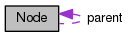
\includegraphics[width=169pt]{classNode__coll__graph}
\end{center}
\end{figure}
\subsection*{Public Member Functions}
\begin{DoxyCompactItemize}
\item 
\hyperlink{classNode_ad7a34779cad45d997bfd6d3d8043c75f}{Node} ()
\item 
\hyperlink{classNode_a2d13f7f1172705cddb79039c2fabbba6}{Node} (int x, int y, \hyperlink{classNode}{Node} $\ast$\+\_\+parent=0, int t=0)
\item 
int \hyperlink{classNode_a81aba8cc7d7ebd60051bb7cba210f587}{getx\+Pos} () const 
\item 
int \hyperlink{classNode_a7d26325d2355b29184cd6b428a78508b}{gety\+Pos} () const 
\item 
float \hyperlink{classNode_ab72b743b5abe69381e9066f4225793d2}{getG} () const 
\item 
float \hyperlink{classNode_ae6f0fa0586f0bba0a33ec57323849d89}{getH} () const 
\item 
float \hyperlink{classNode_ad22eea937020953945d47dc25667baf3}{getF} () const 
\item 
\hyperlink{classNode}{Node} $\ast$ \hyperlink{classNode_aee7fa50380cd3d5fd82c022e45ba2d37}{get\+Parent} () const 
\item 
void \hyperlink{classNode_a95d9ff38e9706097f752df46e1c912d9}{setx\+Pos} (int)
\item 
void \hyperlink{classNode_afcef18b84545fc9097c67ba6b48f31cb}{sety\+Pos} (int)
\item 
void \hyperlink{classNode_ac269852dd9117461a6069589470c39f1}{setG} (float)
\item 
void \hyperlink{classNode_aa10f28d0b00917bc5106373c73eb636f}{setH} (\hyperlink{classNode}{Node} $\ast$meta)
\item 
void \hyperlink{classNode_a77ef44966d6056821545f6b8acee2031}{setF} (float)
\item 
void \hyperlink{classNode_aaed3b50ac429bae4e3460f19c23a9f71}{set\+Parent} (\hyperlink{classNode}{Node} $\ast$)
\item 
void \hyperlink{classNode_aedfbcdc45d98f312e507e34e18b26093}{calculaF} ()
\end{DoxyCompactItemize}
\subsection*{Public Attributes}
\begin{DoxyCompactItemize}
\item 
int \hyperlink{classNode_ab61bfe3b52ba63f10939bf88270321e0}{tamanho}
\item 
int \hyperlink{classNode_a59a543130a10c95f1e8642cf8c5645e8}{id}
\item 
\hyperlink{classNode}{Node} $\ast$ \hyperlink{classNode_ad8184598cdea70e4bbdfd76f2b0f9e85}{parent}
\end{DoxyCompactItemize}
\subsection*{Private Attributes}
\begin{DoxyCompactItemize}
\item 
int \hyperlink{classNode_a4c5b1e397eba5f462edc72d5c031b33e}{x\+Pos}
\item 
int \hyperlink{classNode_ace45ec1cc1cc78ef699918a7adeb1dad}{y\+Pos}
\item 
float \hyperlink{classNode_a3c6a67023068f762eaaa8a4861ab3e9f}{G}
\item 
float \hyperlink{classNode_a26426055f336a81dc05680b981e4c270}{H}
\item 
float \hyperlink{classNode_aa68bc86c2839aca9c05e43541dc973a5}{F}
\end{DoxyCompactItemize}


\subsection{Constructor \& Destructor Documentation}
\index{Node@{Node}!Node@{Node}}
\index{Node@{Node}!Node@{Node}}
\subsubsection[{\texorpdfstring{Node()}{Node()}}]{\setlength{\rightskip}{0pt plus 5cm}Node\+::\+Node (
\begin{DoxyParamCaption}
{}
\end{DoxyParamCaption}
)\hspace{0.3cm}{\ttfamily [inline]}}\hypertarget{classNode_ad7a34779cad45d997bfd6d3d8043c75f}{}\label{classNode_ad7a34779cad45d997bfd6d3d8043c75f}

\begin{DoxyCode}
19 : \hyperlink{classNode_ad8184598cdea70e4bbdfd76f2b0f9e85}{parent}(0) \{\}
\end{DoxyCode}
\index{Node@{Node}!Node@{Node}}
\index{Node@{Node}!Node@{Node}}
\subsubsection[{\texorpdfstring{Node(int x, int y, Node $\ast$\+\_\+parent=0, int t=0)}{Node(int x, int y, Node *_parent=0, int t=0)}}]{\setlength{\rightskip}{0pt plus 5cm}Node\+::\+Node (
\begin{DoxyParamCaption}
\item[{int}]{x, }
\item[{int}]{y, }
\item[{{\bf Node} $\ast$}]{\+\_\+parent = {\ttfamily 0}, }
\item[{int}]{t = {\ttfamily 0}}
\end{DoxyParamCaption}
)\hspace{0.3cm}{\ttfamily [inline]}}\hypertarget{classNode_a2d13f7f1172705cddb79039c2fabbba6}{}\label{classNode_a2d13f7f1172705cddb79039c2fabbba6}

\begin{DoxyCode}
22 : \hyperlink{classNode_a4c5b1e397eba5f462edc72d5c031b33e}{xPos}(x),\hyperlink{classNode_ace45ec1cc1cc78ef699918a7adeb1dad}{yPos}(y),\hyperlink{classNode_a3c6a67023068f762eaaa8a4861ab3e9f}{G}(0),\hyperlink{classNode_a26426055f336a81dc05680b981e4c270}{H}(0),\hyperlink{classNode_ab61bfe3b52ba63f10939bf88270321e0}{tamanho}(t),\hyperlink{classNode_a59a543130a10c95f1e8642cf8c5645e8}{id}(y*\hyperlink{classNode_ab61bfe3b52ba63f10939bf88270321e0}{tamanho}+x),
      \hyperlink{classNode_ad8184598cdea70e4bbdfd76f2b0f9e85}{parent}(\_parent)\{\};
\end{DoxyCode}


Here is the call graph for this function\+:
\nopagebreak
\begin{figure}[H]
\begin{center}
\leavevmode
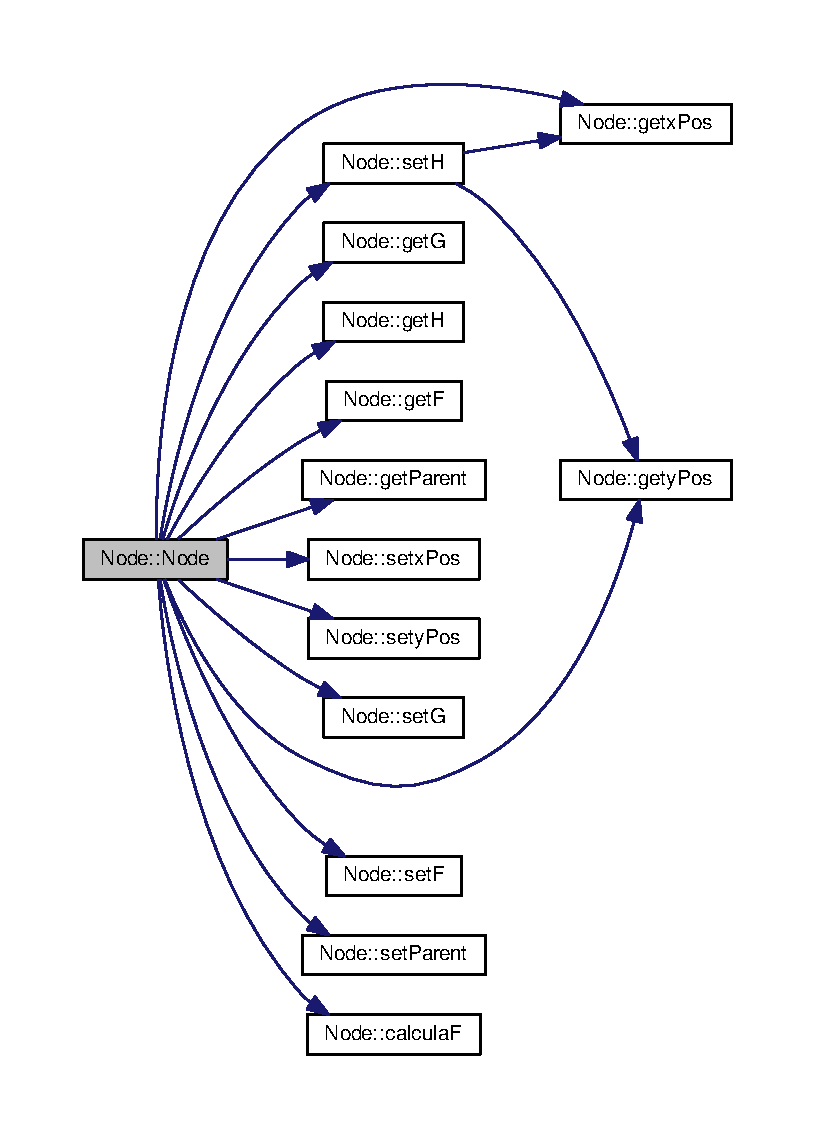
\includegraphics[width=350pt]{classNode_a2d13f7f1172705cddb79039c2fabbba6_cgraph}
\end{center}
\end{figure}




\subsection{Member Function Documentation}
\index{Node@{Node}!calculaF@{calculaF}}
\index{calculaF@{calculaF}!Node@{Node}}
\subsubsection[{\texorpdfstring{calcula\+F()}{calculaF()}}]{\setlength{\rightskip}{0pt plus 5cm}void Node\+::calculaF (
\begin{DoxyParamCaption}
{}
\end{DoxyParamCaption}
)}\hypertarget{classNode_aedfbcdc45d98f312e507e34e18b26093}{}\label{classNode_aedfbcdc45d98f312e507e34e18b26093}

\begin{DoxyCode}
109 \{
110     this->\hyperlink{classNode_aa68bc86c2839aca9c05e43541dc973a5}{F} = this->\hyperlink{classNode_a3c6a67023068f762eaaa8a4861ab3e9f}{G} + this->\hyperlink{classNode_a26426055f336a81dc05680b981e4c270}{H};
111 \}
\end{DoxyCode}
\index{Node@{Node}!getF@{getF}}
\index{getF@{getF}!Node@{Node}}
\subsubsection[{\texorpdfstring{get\+F() const }{getF() const }}]{\setlength{\rightskip}{0pt plus 5cm}float Node\+::getF (
\begin{DoxyParamCaption}
{}
\end{DoxyParamCaption}
) const}\hypertarget{classNode_ad22eea937020953945d47dc25667baf3}{}\label{classNode_ad22eea937020953945d47dc25667baf3}

\begin{DoxyCode}
76 \{
77     \textcolor{keywordflow}{return} this->\hyperlink{classNode_aa68bc86c2839aca9c05e43541dc973a5}{F};
78 \}
\end{DoxyCode}
\index{Node@{Node}!getG@{getG}}
\index{getG@{getG}!Node@{Node}}
\subsubsection[{\texorpdfstring{get\+G() const }{getG() const }}]{\setlength{\rightskip}{0pt plus 5cm}float Node\+::getG (
\begin{DoxyParamCaption}
{}
\end{DoxyParamCaption}
) const}\hypertarget{classNode_ab72b743b5abe69381e9066f4225793d2}{}\label{classNode_ab72b743b5abe69381e9066f4225793d2}

\begin{DoxyCode}
68 \{
69     \textcolor{keywordflow}{return} this->\hyperlink{classNode_a3c6a67023068f762eaaa8a4861ab3e9f}{G}; 
70 \}
\end{DoxyCode}
\index{Node@{Node}!getH@{getH}}
\index{getH@{getH}!Node@{Node}}
\subsubsection[{\texorpdfstring{get\+H() const }{getH() const }}]{\setlength{\rightskip}{0pt plus 5cm}float Node\+::getH (
\begin{DoxyParamCaption}
{}
\end{DoxyParamCaption}
) const}\hypertarget{classNode_ae6f0fa0586f0bba0a33ec57323849d89}{}\label{classNode_ae6f0fa0586f0bba0a33ec57323849d89}

\begin{DoxyCode}
72 \{
73     \textcolor{keywordflow}{return} this->\hyperlink{classNode_a26426055f336a81dc05680b981e4c270}{H};
74 \}
\end{DoxyCode}
\index{Node@{Node}!get\+Parent@{get\+Parent}}
\index{get\+Parent@{get\+Parent}!Node@{Node}}
\subsubsection[{\texorpdfstring{get\+Parent() const }{getParent() const }}]{\setlength{\rightskip}{0pt plus 5cm}{\bf Node} $\ast$ Node\+::get\+Parent (
\begin{DoxyParamCaption}
{}
\end{DoxyParamCaption}
) const}\hypertarget{classNode_aee7fa50380cd3d5fd82c022e45ba2d37}{}\label{classNode_aee7fa50380cd3d5fd82c022e45ba2d37}

\begin{DoxyCode}
80 \{
81     \textcolor{keywordflow}{return} this->\hyperlink{classNode_ad8184598cdea70e4bbdfd76f2b0f9e85}{parent};
82 \}
\end{DoxyCode}
\index{Node@{Node}!getx\+Pos@{getx\+Pos}}
\index{getx\+Pos@{getx\+Pos}!Node@{Node}}
\subsubsection[{\texorpdfstring{getx\+Pos() const }{getxPos() const }}]{\setlength{\rightskip}{0pt plus 5cm}int Node\+::getx\+Pos (
\begin{DoxyParamCaption}
{}
\end{DoxyParamCaption}
) const}\hypertarget{classNode_a81aba8cc7d7ebd60051bb7cba210f587}{}\label{classNode_a81aba8cc7d7ebd60051bb7cba210f587}

\begin{DoxyCode}
60 \{
61     \textcolor{keywordflow}{return} this->\hyperlink{classNode_a4c5b1e397eba5f462edc72d5c031b33e}{xPos};
62 \}
\end{DoxyCode}
\index{Node@{Node}!gety\+Pos@{gety\+Pos}}
\index{gety\+Pos@{gety\+Pos}!Node@{Node}}
\subsubsection[{\texorpdfstring{gety\+Pos() const }{getyPos() const }}]{\setlength{\rightskip}{0pt plus 5cm}int Node\+::gety\+Pos (
\begin{DoxyParamCaption}
{}
\end{DoxyParamCaption}
) const}\hypertarget{classNode_a7d26325d2355b29184cd6b428a78508b}{}\label{classNode_a7d26325d2355b29184cd6b428a78508b}

\begin{DoxyCode}
64 \{
65     \textcolor{keywordflow}{return} this->\hyperlink{classNode_ace45ec1cc1cc78ef699918a7adeb1dad}{yPos};
66 \}
\end{DoxyCode}
\index{Node@{Node}!setF@{setF}}
\index{setF@{setF}!Node@{Node}}
\subsubsection[{\texorpdfstring{set\+F(float)}{setF(float)}}]{\setlength{\rightskip}{0pt plus 5cm}void Node\+::setF (
\begin{DoxyParamCaption}
\item[{float}]{F}
\end{DoxyParamCaption}
)}\hypertarget{classNode_a77ef44966d6056821545f6b8acee2031}{}\label{classNode_a77ef44966d6056821545f6b8acee2031}

\begin{DoxyCode}
101 \{
102     this->\hyperlink{classNode_aa68bc86c2839aca9c05e43541dc973a5}{F} = \hyperlink{classNode_aa68bc86c2839aca9c05e43541dc973a5}{F};
103 \}
\end{DoxyCode}
\index{Node@{Node}!setG@{setG}}
\index{setG@{setG}!Node@{Node}}
\subsubsection[{\texorpdfstring{set\+G(float)}{setG(float)}}]{\setlength{\rightskip}{0pt plus 5cm}void Node\+::setG (
\begin{DoxyParamCaption}
\item[{float}]{G}
\end{DoxyParamCaption}
)}\hypertarget{classNode_ac269852dd9117461a6069589470c39f1}{}\label{classNode_ac269852dd9117461a6069589470c39f1}

\begin{DoxyCode}
93 \{
94     this->\hyperlink{classNode_a3c6a67023068f762eaaa8a4861ab3e9f}{G} = \hyperlink{classNode_a3c6a67023068f762eaaa8a4861ab3e9f}{G};
95 \}
\end{DoxyCode}
\index{Node@{Node}!setH@{setH}}
\index{setH@{setH}!Node@{Node}}
\subsubsection[{\texorpdfstring{set\+H(\+Node $\ast$meta)}{setH(Node *meta)}}]{\setlength{\rightskip}{0pt plus 5cm}void Node\+::setH (
\begin{DoxyParamCaption}
\item[{{\bf Node} $\ast$}]{meta}
\end{DoxyParamCaption}
)}\hypertarget{classNode_aa10f28d0b00917bc5106373c73eb636f}{}\label{classNode_aa10f28d0b00917bc5106373c73eb636f}

\begin{DoxyCode}
97 \{
98     this->\hyperlink{classNode_a26426055f336a81dc05680b981e4c270}{H} = (sqrt(((meta->\hyperlink{classNode_a81aba8cc7d7ebd60051bb7cba210f587}{getxPos}()-this->\hyperlink{classNode_a4c5b1e397eba5f462edc72d5c031b33e}{xPos})*(meta->\hyperlink{classNode_a81aba8cc7d7ebd60051bb7cba210f587}{getxPos}()-this->
      \hyperlink{classNode_a4c5b1e397eba5f462edc72d5c031b33e}{xPos}))+((meta->\hyperlink{classNode_a7d26325d2355b29184cd6b428a78508b}{getyPos}()-this->\hyperlink{classNode_ace45ec1cc1cc78ef699918a7adeb1dad}{yPos})*(meta->\hyperlink{classNode_a7d26325d2355b29184cd6b428a78508b}{getyPos}()-this->
      \hyperlink{classNode_ace45ec1cc1cc78ef699918a7adeb1dad}{yPos}))));
99 \}
\end{DoxyCode}


Here is the call graph for this function\+:
\nopagebreak
\begin{figure}[H]
\begin{center}
\leavevmode
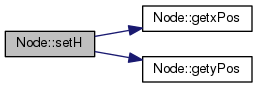
\includegraphics[width=265pt]{classNode_aa10f28d0b00917bc5106373c73eb636f_cgraph}
\end{center}
\end{figure}


\index{Node@{Node}!set\+Parent@{set\+Parent}}
\index{set\+Parent@{set\+Parent}!Node@{Node}}
\subsubsection[{\texorpdfstring{set\+Parent(\+Node $\ast$)}{setParent(Node *)}}]{\setlength{\rightskip}{0pt plus 5cm}void Node\+::set\+Parent (
\begin{DoxyParamCaption}
\item[{{\bf Node} $\ast$}]{parent}
\end{DoxyParamCaption}
)}\hypertarget{classNode_aaed3b50ac429bae4e3460f19c23a9f71}{}\label{classNode_aaed3b50ac429bae4e3460f19c23a9f71}

\begin{DoxyCode}
105 \{
106     this->parent = \hyperlink{classNode_ad8184598cdea70e4bbdfd76f2b0f9e85}{parent};
107 \}
\end{DoxyCode}
\index{Node@{Node}!setx\+Pos@{setx\+Pos}}
\index{setx\+Pos@{setx\+Pos}!Node@{Node}}
\subsubsection[{\texorpdfstring{setx\+Pos(int)}{setxPos(int)}}]{\setlength{\rightskip}{0pt plus 5cm}void Node\+::setx\+Pos (
\begin{DoxyParamCaption}
\item[{int}]{x}
\end{DoxyParamCaption}
)}\hypertarget{classNode_a95d9ff38e9706097f752df46e1c912d9}{}\label{classNode_a95d9ff38e9706097f752df46e1c912d9}

\begin{DoxyCode}
85 \{
86     this->\hyperlink{classNode_a4c5b1e397eba5f462edc72d5c031b33e}{xPos} = x;
87 \}
\end{DoxyCode}
\index{Node@{Node}!sety\+Pos@{sety\+Pos}}
\index{sety\+Pos@{sety\+Pos}!Node@{Node}}
\subsubsection[{\texorpdfstring{sety\+Pos(int)}{setyPos(int)}}]{\setlength{\rightskip}{0pt plus 5cm}void Node\+::sety\+Pos (
\begin{DoxyParamCaption}
\item[{int}]{y}
\end{DoxyParamCaption}
)}\hypertarget{classNode_afcef18b84545fc9097c67ba6b48f31cb}{}\label{classNode_afcef18b84545fc9097c67ba6b48f31cb}

\begin{DoxyCode}
89 \{
90     this->\hyperlink{classNode_ace45ec1cc1cc78ef699918a7adeb1dad}{yPos} = y;
91 \}
\end{DoxyCode}


\subsection{Member Data Documentation}
\index{Node@{Node}!F@{F}}
\index{F@{F}!Node@{Node}}
\subsubsection[{\texorpdfstring{F}{F}}]{\setlength{\rightskip}{0pt plus 5cm}float Node\+::F\hspace{0.3cm}{\ttfamily [private]}}\hypertarget{classNode_aa68bc86c2839aca9c05e43541dc973a5}{}\label{classNode_aa68bc86c2839aca9c05e43541dc973a5}
\index{Node@{Node}!G@{G}}
\index{G@{G}!Node@{Node}}
\subsubsection[{\texorpdfstring{G}{G}}]{\setlength{\rightskip}{0pt plus 5cm}float Node\+::G\hspace{0.3cm}{\ttfamily [private]}}\hypertarget{classNode_a3c6a67023068f762eaaa8a4861ab3e9f}{}\label{classNode_a3c6a67023068f762eaaa8a4861ab3e9f}
\index{Node@{Node}!H@{H}}
\index{H@{H}!Node@{Node}}
\subsubsection[{\texorpdfstring{H}{H}}]{\setlength{\rightskip}{0pt plus 5cm}float Node\+::H\hspace{0.3cm}{\ttfamily [private]}}\hypertarget{classNode_a26426055f336a81dc05680b981e4c270}{}\label{classNode_a26426055f336a81dc05680b981e4c270}
\index{Node@{Node}!id@{id}}
\index{id@{id}!Node@{Node}}
\subsubsection[{\texorpdfstring{id}{id}}]{\setlength{\rightskip}{0pt plus 5cm}int Node\+::id}\hypertarget{classNode_a59a543130a10c95f1e8642cf8c5645e8}{}\label{classNode_a59a543130a10c95f1e8642cf8c5645e8}
\index{Node@{Node}!parent@{parent}}
\index{parent@{parent}!Node@{Node}}
\subsubsection[{\texorpdfstring{parent}{parent}}]{\setlength{\rightskip}{0pt plus 5cm}{\bf Node}$\ast$ Node\+::parent}\hypertarget{classNode_ad8184598cdea70e4bbdfd76f2b0f9e85}{}\label{classNode_ad8184598cdea70e4bbdfd76f2b0f9e85}
\index{Node@{Node}!tamanho@{tamanho}}
\index{tamanho@{tamanho}!Node@{Node}}
\subsubsection[{\texorpdfstring{tamanho}{tamanho}}]{\setlength{\rightskip}{0pt plus 5cm}int Node\+::tamanho}\hypertarget{classNode_ab61bfe3b52ba63f10939bf88270321e0}{}\label{classNode_ab61bfe3b52ba63f10939bf88270321e0}
\index{Node@{Node}!x\+Pos@{x\+Pos}}
\index{x\+Pos@{x\+Pos}!Node@{Node}}
\subsubsection[{\texorpdfstring{x\+Pos}{xPos}}]{\setlength{\rightskip}{0pt plus 5cm}int Node\+::x\+Pos\hspace{0.3cm}{\ttfamily [private]}}\hypertarget{classNode_a4c5b1e397eba5f462edc72d5c031b33e}{}\label{classNode_a4c5b1e397eba5f462edc72d5c031b33e}
\index{Node@{Node}!y\+Pos@{y\+Pos}}
\index{y\+Pos@{y\+Pos}!Node@{Node}}
\subsubsection[{\texorpdfstring{y\+Pos}{yPos}}]{\setlength{\rightskip}{0pt plus 5cm}int Node\+::y\+Pos\hspace{0.3cm}{\ttfamily [private]}}\hypertarget{classNode_ace45ec1cc1cc78ef699918a7adeb1dad}{}\label{classNode_ace45ec1cc1cc78ef699918a7adeb1dad}


The documentation for this class was generated from the following files\+:\begin{DoxyCompactItemize}
\item 
\hyperlink{CalculoTempo__node_8h}{Calculo\+Tempo\+\_\+node.\+h}\item 
\hyperlink{CalculoTempo__node_8cpp}{Calculo\+Tempo\+\_\+node.\+cpp}\end{DoxyCompactItemize}

\hypertarget{classStudent}{}\section{Student Class Reference}
\label{classStudent}\index{Student@{Student}}


{\ttfamily \#include $<$Student.\+h$>$}

\subsection*{Public Member Functions}
\begin{DoxyCompactItemize}
\item 
\hyperlink{classStudent_af9168cedbfa5565cf0b20c1a9d3f5c9d}{Student} ()
\item 
\hyperlink{classStudent_a557917f9af87042e5fa25bd7b1aeaa30}{Student} (string f, string l, char m, int s, int a)
\item 
\hyperlink{classStudent_a9b3d40ac356f6794eeae74ce473a5617}{Student} (const \hyperlink{classStudent}{Student} \&s)
\item 
void \hyperlink{classStudent_a30731c688a4d7e3c047605de86c78007}{set\+Name} (string f, string l, char m)
\item 
void \hyperlink{classStudent_a46dafabdf7259d22c2ed038d187018d6}{set\+S\+SN} (int s)
\item 
void \hyperlink{classStudent_aae26ec99b719c86b60b33e19bc4f3986}{set\+Age} (int a)
\item 
string \hyperlink{classStudent_ac0c4ea968202c325e11b33ef38087701}{get\+First\+Name} () const 
\item 
string \hyperlink{classStudent_ae58e20cf8d78eecdbbd34c04f7a2c846}{get\+Last\+Name} () const 
\item 
char \hyperlink{classStudent_a9f266c04ecea344e544f9e772921d17c}{get\+Middle\+Initial} () const 
\item 
int \hyperlink{classStudent_acb222ca39f470aaa1562a25d329e8378}{get\+S\+SN} () const 
\item 
int \hyperlink{classStudent_a05e941545afe646579a8e91dfc8f1953}{get\+Age} () const 
\item 
void \hyperlink{classStudent_afeae2ddd8936ba4f37064a8d751f51eb}{read} (istream \&in)
\item 
void \hyperlink{classStudent_a17a6f00e4ec4637f77a50c2769e69721}{print} (ostream \&out)
\item 
bool \hyperlink{classStudent_a3f82e382259835b187fd92f2b15fcb42}{operator$>$} (const \hyperlink{classStudent}{Student} \&s) const 
\item 
bool \hyperlink{classStudent_a4add57e859306b4a543368201ca0922f}{operator$<$} (const \hyperlink{classStudent}{Student} \&s) const 
\end{DoxyCompactItemize}
\subsection*{Private Attributes}
\begin{DoxyCompactItemize}
\item 
string \hyperlink{classStudent_a333c7d227c87fdfa821d0232e21f9006}{fname}
\item 
string \hyperlink{classStudent_a6c934004d6a468a354916bcf0f998190}{lname}
\item 
char \hyperlink{classStudent_afd8d4557f2ac6bb7681c32e691248328}{mi}
\item 
int \hyperlink{classStudent_aa7181a8aac86888176481f901bee2cbd}{ssn}
\item 
int \hyperlink{classStudent_a552a431a43ffc545d180424597d51f97}{age}
\end{DoxyCompactItemize}
\subsection*{Friends}
\begin{DoxyCompactItemize}
\item 
class \hyperlink{classStudent_a6db9d28bd448a131448276ee03de1e6d}{Node}
\item 
ostream \& \hyperlink{classStudent_a8ed16acc8384ea29641694cb182ac764}{operator$<$$<$} (ostream \&outs, const \hyperlink{classStudent}{Student} \&s)
\item 
istream \& \hyperlink{classStudent_a2d76cee765e6e0d66e66a27d10fa0a68}{operator$>$$>$} (istream \&ins, \hyperlink{classStudent}{Student} \&s)
\end{DoxyCompactItemize}


\subsection{Constructor \& Destructor Documentation}
\index{Student@{Student}!Student@{Student}}
\index{Student@{Student}!Student@{Student}}
\subsubsection[{\texorpdfstring{Student()}{Student()}}]{\setlength{\rightskip}{0pt plus 5cm}Student\+::\+Student (
\begin{DoxyParamCaption}
{}
\end{DoxyParamCaption}
)\hspace{0.3cm}{\ttfamily [inline]}}\hypertarget{classStudent_af9168cedbfa5565cf0b20c1a9d3f5c9d}{}\label{classStudent_af9168cedbfa5565cf0b20c1a9d3f5c9d}

\begin{DoxyCode}
32 : \hyperlink{classStudent_a333c7d227c87fdfa821d0232e21f9006}{fname}(\textcolor{stringliteral}{""}), \hyperlink{classStudent_a6c934004d6a468a354916bcf0f998190}{lname}(\textcolor{stringliteral}{""}), \hyperlink{classStudent_afd8d4557f2ac6bb7681c32e691248328}{mi}(\textcolor{charliteral}{' '}), \hyperlink{classStudent_aa7181a8aac86888176481f901bee2cbd}{ssn}(0), \hyperlink{classStudent_a552a431a43ffc545d180424597d51f97}{age}(0) \{\} \textcolor{comment}{//default constructor                 
                                                                                                             }
\end{DoxyCode}
\index{Student@{Student}!Student@{Student}}
\index{Student@{Student}!Student@{Student}}
\subsubsection[{\texorpdfstring{Student(string f, string l, char m, int s, int a)}{Student(string f, string l, char m, int s, int a)}}]{\setlength{\rightskip}{0pt plus 5cm}Student\+::\+Student (
\begin{DoxyParamCaption}
\item[{string}]{f, }
\item[{string}]{l, }
\item[{char}]{m, }
\item[{int}]{s, }
\item[{int}]{a}
\end{DoxyParamCaption}
)\hspace{0.3cm}{\ttfamily [inline]}}\hypertarget{classStudent_a557917f9af87042e5fa25bd7b1aeaa30}{}\label{classStudent_a557917f9af87042e5fa25bd7b1aeaa30}

\begin{DoxyCode}
33 : \hyperlink{classStudent_a333c7d227c87fdfa821d0232e21f9006}{fname}(f), \hyperlink{classStudent_a6c934004d6a468a354916bcf0f998190}{lname}(l), \hyperlink{classStudent_afd8d4557f2ac6bb7681c32e691248328}{mi}(m), \hyperlink{classStudent_aa7181a8aac86888176481f901bee2cbd}{ssn}(s), \hyperlink{classStudent_a552a431a43ffc545d180424597d51f97}{age}(a) \{\}
\end{DoxyCode}
\index{Student@{Student}!Student@{Student}}
\index{Student@{Student}!Student@{Student}}
\subsubsection[{\texorpdfstring{Student(const Student \&s)}{Student(const Student &s)}}]{\setlength{\rightskip}{0pt plus 5cm}Student\+::\+Student (
\begin{DoxyParamCaption}
\item[{const {\bf Student} \&}]{s}
\end{DoxyParamCaption}
)}\hypertarget{classStudent_a9b3d40ac356f6794eeae74ce473a5617}{}\label{classStudent_a9b3d40ac356f6794eeae74ce473a5617}

\begin{DoxyCode}
14 \{
15    \hyperlink{classStudent_a333c7d227c87fdfa821d0232e21f9006}{fname} = s.\hyperlink{classStudent_a333c7d227c87fdfa821d0232e21f9006}{fname};
16    \hyperlink{classStudent_a6c934004d6a468a354916bcf0f998190}{lname} = s.\hyperlink{classStudent_a6c934004d6a468a354916bcf0f998190}{lname};
17    \hyperlink{classStudent_afd8d4557f2ac6bb7681c32e691248328}{mi} = s.\hyperlink{classStudent_afd8d4557f2ac6bb7681c32e691248328}{mi};
18    \hyperlink{classStudent_aa7181a8aac86888176481f901bee2cbd}{ssn} = s.\hyperlink{classStudent_aa7181a8aac86888176481f901bee2cbd}{ssn};
19    \hyperlink{classStudent_a552a431a43ffc545d180424597d51f97}{age} = s.\hyperlink{classStudent_a552a431a43ffc545d180424597d51f97}{age};
20 \}
\end{DoxyCode}


\subsection{Member Function Documentation}
\index{Student@{Student}!get\+Age@{get\+Age}}
\index{get\+Age@{get\+Age}!Student@{Student}}
\subsubsection[{\texorpdfstring{get\+Age() const }{getAge() const }}]{\setlength{\rightskip}{0pt plus 5cm}int Student\+::get\+Age (
\begin{DoxyParamCaption}
{}
\end{DoxyParamCaption}
) const}\hypertarget{classStudent_a05e941545afe646579a8e91dfc8f1953}{}\label{classStudent_a05e941545afe646579a8e91dfc8f1953}

\begin{DoxyCode}
60 \{
61    \textcolor{keywordflow}{return} \hyperlink{classStudent_a552a431a43ffc545d180424597d51f97}{age};
62 \}
\end{DoxyCode}
\index{Student@{Student}!get\+First\+Name@{get\+First\+Name}}
\index{get\+First\+Name@{get\+First\+Name}!Student@{Student}}
\subsubsection[{\texorpdfstring{get\+First\+Name() const }{getFirstName() const }}]{\setlength{\rightskip}{0pt plus 5cm}string Student\+::get\+First\+Name (
\begin{DoxyParamCaption}
{}
\end{DoxyParamCaption}
) const}\hypertarget{classStudent_ac0c4ea968202c325e11b33ef38087701}{}\label{classStudent_ac0c4ea968202c325e11b33ef38087701}

\begin{DoxyCode}
40 \{
41    \textcolor{keywordflow}{return} \hyperlink{classStudent_a333c7d227c87fdfa821d0232e21f9006}{fname};
42 \}
\end{DoxyCode}
\index{Student@{Student}!get\+Last\+Name@{get\+Last\+Name}}
\index{get\+Last\+Name@{get\+Last\+Name}!Student@{Student}}
\subsubsection[{\texorpdfstring{get\+Last\+Name() const }{getLastName() const }}]{\setlength{\rightskip}{0pt plus 5cm}string Student\+::get\+Last\+Name (
\begin{DoxyParamCaption}
{}
\end{DoxyParamCaption}
) const}\hypertarget{classStudent_ae58e20cf8d78eecdbbd34c04f7a2c846}{}\label{classStudent_ae58e20cf8d78eecdbbd34c04f7a2c846}

\begin{DoxyCode}
45 \{
46    \textcolor{keywordflow}{return} \hyperlink{classStudent_a6c934004d6a468a354916bcf0f998190}{lname};
47 \}
\end{DoxyCode}
\index{Student@{Student}!get\+Middle\+Initial@{get\+Middle\+Initial}}
\index{get\+Middle\+Initial@{get\+Middle\+Initial}!Student@{Student}}
\subsubsection[{\texorpdfstring{get\+Middle\+Initial() const }{getMiddleInitial() const }}]{\setlength{\rightskip}{0pt plus 5cm}char Student\+::get\+Middle\+Initial (
\begin{DoxyParamCaption}
{}
\end{DoxyParamCaption}
) const}\hypertarget{classStudent_a9f266c04ecea344e544f9e772921d17c}{}\label{classStudent_a9f266c04ecea344e544f9e772921d17c}

\begin{DoxyCode}
50 \{
51    \textcolor{keywordflow}{return} \hyperlink{classStudent_afd8d4557f2ac6bb7681c32e691248328}{mi};
52 \}
\end{DoxyCode}
\index{Student@{Student}!get\+S\+SN@{get\+S\+SN}}
\index{get\+S\+SN@{get\+S\+SN}!Student@{Student}}
\subsubsection[{\texorpdfstring{get\+S\+S\+N() const }{getSSN() const }}]{\setlength{\rightskip}{0pt plus 5cm}int Student\+::get\+S\+SN (
\begin{DoxyParamCaption}
{}
\end{DoxyParamCaption}
) const}\hypertarget{classStudent_acb222ca39f470aaa1562a25d329e8378}{}\label{classStudent_acb222ca39f470aaa1562a25d329e8378}

\begin{DoxyCode}
55 \{
56    \textcolor{keywordflow}{return} \hyperlink{classStudent_aa7181a8aac86888176481f901bee2cbd}{ssn};
57 \}
\end{DoxyCode}
\index{Student@{Student}!operator$<$@{operator$<$}}
\index{operator$<$@{operator$<$}!Student@{Student}}
\subsubsection[{\texorpdfstring{operator$<$(const Student \&s) const }{operator<(const Student &s) const }}]{\setlength{\rightskip}{0pt plus 5cm}bool Student\+::operator$<$ (
\begin{DoxyParamCaption}
\item[{const {\bf Student} \&}]{s}
\end{DoxyParamCaption}
) const}\hypertarget{classStudent_a4add57e859306b4a543368201ca0922f}{}\label{classStudent_a4add57e859306b4a543368201ca0922f}

\begin{DoxyCode}
94 \{
95    \textcolor{keywordflow}{return} (\hyperlink{classStudent_a6c934004d6a468a354916bcf0f998190}{lname}.compare(s.\hyperlink{classStudent_a6c934004d6a468a354916bcf0f998190}{lname}) < 0);
96 \}\end{DoxyCode}
\index{Student@{Student}!operator$>$@{operator$>$}}
\index{operator$>$@{operator$>$}!Student@{Student}}
\subsubsection[{\texorpdfstring{operator$>$(const Student \&s) const }{operator>(const Student &s) const }}]{\setlength{\rightskip}{0pt plus 5cm}bool Student\+::operator$>$ (
\begin{DoxyParamCaption}
\item[{const {\bf Student} \&}]{s}
\end{DoxyParamCaption}
) const}\hypertarget{classStudent_a3f82e382259835b187fd92f2b15fcb42}{}\label{classStudent_a3f82e382259835b187fd92f2b15fcb42}

\begin{DoxyCode}
89 \{
90    \textcolor{keywordflow}{return} (\hyperlink{classStudent_a6c934004d6a468a354916bcf0f998190}{lname}.compare(s.\hyperlink{classStudent_a6c934004d6a468a354916bcf0f998190}{lname}) > 0);
91 \}
\end{DoxyCode}
\index{Student@{Student}!print@{print}}
\index{print@{print}!Student@{Student}}
\subsubsection[{\texorpdfstring{print(ostream \&out)}{print(ostream &out)}}]{\setlength{\rightskip}{0pt plus 5cm}void Student\+::print (
\begin{DoxyParamCaption}
\item[{ostream \&}]{out}
\end{DoxyParamCaption}
)}\hypertarget{classStudent_a17a6f00e4ec4637f77a50c2769e69721}{}\label{classStudent_a17a6f00e4ec4637f77a50c2769e69721}

\begin{DoxyCode}
80 \{
81    out << \hyperlink{classStudent_a333c7d227c87fdfa821d0232e21f9006}{fname} << endl;
82    out << \hyperlink{classStudent_a6c934004d6a468a354916bcf0f998190}{lname} << endl;
83    out << \hyperlink{classStudent_afd8d4557f2ac6bb7681c32e691248328}{mi} << endl;
84    out << \hyperlink{classStudent_aa7181a8aac86888176481f901bee2cbd}{ssn} << endl;
85    out << \hyperlink{classStudent_a552a431a43ffc545d180424597d51f97}{age} << endl;
86 \}
\end{DoxyCode}
\index{Student@{Student}!read@{read}}
\index{read@{read}!Student@{Student}}
\subsubsection[{\texorpdfstring{read(istream \&in)}{read(istream &in)}}]{\setlength{\rightskip}{0pt plus 5cm}void Student\+::read (
\begin{DoxyParamCaption}
\item[{istream \&}]{in}
\end{DoxyParamCaption}
)}\hypertarget{classStudent_afeae2ddd8936ba4f37064a8d751f51eb}{}\label{classStudent_afeae2ddd8936ba4f37064a8d751f51eb}
\index{Student@{Student}!set\+Age@{set\+Age}}
\index{set\+Age@{set\+Age}!Student@{Student}}
\subsubsection[{\texorpdfstring{set\+Age(int a)}{setAge(int a)}}]{\setlength{\rightskip}{0pt plus 5cm}void Student\+::set\+Age (
\begin{DoxyParamCaption}
\item[{int}]{a}
\end{DoxyParamCaption}
)}\hypertarget{classStudent_aae26ec99b719c86b60b33e19bc4f3986}{}\label{classStudent_aae26ec99b719c86b60b33e19bc4f3986}

\begin{DoxyCode}
35 \{
36    \hyperlink{classStudent_a552a431a43ffc545d180424597d51f97}{age} = a;
37 \}
\end{DoxyCode}
\index{Student@{Student}!set\+Name@{set\+Name}}
\index{set\+Name@{set\+Name}!Student@{Student}}
\subsubsection[{\texorpdfstring{set\+Name(string f, string l, char m)}{setName(string f, string l, char m)}}]{\setlength{\rightskip}{0pt plus 5cm}void Student\+::set\+Name (
\begin{DoxyParamCaption}
\item[{string}]{f, }
\item[{string}]{l, }
\item[{char}]{m}
\end{DoxyParamCaption}
)}\hypertarget{classStudent_a30731c688a4d7e3c047605de86c78007}{}\label{classStudent_a30731c688a4d7e3c047605de86c78007}

\begin{DoxyCode}
23 \{
24    \hyperlink{classStudent_a333c7d227c87fdfa821d0232e21f9006}{fname} = f;
25    \hyperlink{classStudent_a6c934004d6a468a354916bcf0f998190}{lname} = l;
26    \hyperlink{classStudent_afd8d4557f2ac6bb7681c32e691248328}{mi} = m;
27 \}
\end{DoxyCode}
\index{Student@{Student}!set\+S\+SN@{set\+S\+SN}}
\index{set\+S\+SN@{set\+S\+SN}!Student@{Student}}
\subsubsection[{\texorpdfstring{set\+S\+S\+N(int s)}{setSSN(int s)}}]{\setlength{\rightskip}{0pt plus 5cm}void Student\+::set\+S\+SN (
\begin{DoxyParamCaption}
\item[{int}]{s}
\end{DoxyParamCaption}
)}\hypertarget{classStudent_a46dafabdf7259d22c2ed038d187018d6}{}\label{classStudent_a46dafabdf7259d22c2ed038d187018d6}

\begin{DoxyCode}
30 \{
31    \hyperlink{classStudent_aa7181a8aac86888176481f901bee2cbd}{ssn} = s;
32 \}
\end{DoxyCode}


\subsection{Friends And Related Function Documentation}
\index{Student@{Student}!Node@{Node}}
\index{Node@{Node}!Student@{Student}}
\subsubsection[{\texorpdfstring{Node}{Node}}]{\setlength{\rightskip}{0pt plus 5cm}friend class {\bf Node}\hspace{0.3cm}{\ttfamily [friend]}}\hypertarget{classStudent_a6db9d28bd448a131448276ee03de1e6d}{}\label{classStudent_a6db9d28bd448a131448276ee03de1e6d}
\index{Student@{Student}!operator$<$$<$@{operator$<$$<$}}
\index{operator$<$$<$@{operator$<$$<$}!Student@{Student}}
\subsubsection[{\texorpdfstring{operator$<$$<$}{operator<<}}]{\setlength{\rightskip}{0pt plus 5cm}ostream\& operator$<$$<$ (
\begin{DoxyParamCaption}
\item[{ostream \&}]{outs, }
\item[{const {\bf Student} \&}]{s}
\end{DoxyParamCaption}
)\hspace{0.3cm}{\ttfamily [friend]}}\hypertarget{classStudent_a8ed16acc8384ea29641694cb182ac764}{}\label{classStudent_a8ed16acc8384ea29641694cb182ac764}

\begin{DoxyCode}
65 \{
66    cout << \textcolor{stringliteral}{"Student:\(\backslash\)t\(\backslash\)t  "} << s.\hyperlink{classStudent_a6c934004d6a468a354916bcf0f998190}{lname} << \textcolor{stringliteral}{", "} << s.\hyperlink{classStudent_a333c7d227c87fdfa821d0232e21f9006}{fname} << \textcolor{stringliteral}{" "} << s.
      \hyperlink{classStudent_afd8d4557f2ac6bb7681c32e691248328}{mi} << endl;
67    cout << \textcolor{stringliteral}{"Social Security number:\(\backslash\)t  "} << s.\hyperlink{classStudent_aa7181a8aac86888176481f901bee2cbd}{ssn} << endl;
68    cout << \textcolor{stringliteral}{"Age:\(\backslash\)t\(\backslash\)t\(\backslash\)t  "} << s.\hyperlink{classStudent_a552a431a43ffc545d180424597d51f97}{age} << endl;
69    cout << \textcolor{stringliteral}{"------------------------------------------------------"} << endl;
70 
71    \textcolor{keywordflow}{return} outs;
72 \}
\end{DoxyCode}
\index{Student@{Student}!operator$>$$>$@{operator$>$$>$}}
\index{operator$>$$>$@{operator$>$$>$}!Student@{Student}}
\subsubsection[{\texorpdfstring{operator$>$$>$}{operator>>}}]{\setlength{\rightskip}{0pt plus 5cm}istream\& operator$>$$>$ (
\begin{DoxyParamCaption}
\item[{istream \&}]{ins, }
\item[{{\bf Student} \&}]{s}
\end{DoxyParamCaption}
)\hspace{0.3cm}{\ttfamily [friend]}}\hypertarget{classStudent_a2d76cee765e6e0d66e66a27d10fa0a68}{}\label{classStudent_a2d76cee765e6e0d66e66a27d10fa0a68}

\begin{DoxyCode}
75 \{
76    ins >> s.\hyperlink{classStudent_a333c7d227c87fdfa821d0232e21f9006}{fname} >> s.\hyperlink{classStudent_a6c934004d6a468a354916bcf0f998190}{lname} >> s.\hyperlink{classStudent_afd8d4557f2ac6bb7681c32e691248328}{mi} >> s.\hyperlink{classStudent_aa7181a8aac86888176481f901bee2cbd}{ssn} >> s.\hyperlink{classStudent_a552a431a43ffc545d180424597d51f97}{age};
77 \}
\end{DoxyCode}


\subsection{Member Data Documentation}
\index{Student@{Student}!age@{age}}
\index{age@{age}!Student@{Student}}
\subsubsection[{\texorpdfstring{age}{age}}]{\setlength{\rightskip}{0pt plus 5cm}int Student\+::age\hspace{0.3cm}{\ttfamily [private]}}\hypertarget{classStudent_a552a431a43ffc545d180424597d51f97}{}\label{classStudent_a552a431a43ffc545d180424597d51f97}
\index{Student@{Student}!fname@{fname}}
\index{fname@{fname}!Student@{Student}}
\subsubsection[{\texorpdfstring{fname}{fname}}]{\setlength{\rightskip}{0pt plus 5cm}string Student\+::fname\hspace{0.3cm}{\ttfamily [private]}}\hypertarget{classStudent_a333c7d227c87fdfa821d0232e21f9006}{}\label{classStudent_a333c7d227c87fdfa821d0232e21f9006}
\index{Student@{Student}!lname@{lname}}
\index{lname@{lname}!Student@{Student}}
\subsubsection[{\texorpdfstring{lname}{lname}}]{\setlength{\rightskip}{0pt plus 5cm}string Student\+::lname\hspace{0.3cm}{\ttfamily [private]}}\hypertarget{classStudent_a6c934004d6a468a354916bcf0f998190}{}\label{classStudent_a6c934004d6a468a354916bcf0f998190}
\index{Student@{Student}!mi@{mi}}
\index{mi@{mi}!Student@{Student}}
\subsubsection[{\texorpdfstring{mi}{mi}}]{\setlength{\rightskip}{0pt plus 5cm}char Student\+::mi\hspace{0.3cm}{\ttfamily [private]}}\hypertarget{classStudent_afd8d4557f2ac6bb7681c32e691248328}{}\label{classStudent_afd8d4557f2ac6bb7681c32e691248328}
\index{Student@{Student}!ssn@{ssn}}
\index{ssn@{ssn}!Student@{Student}}
\subsubsection[{\texorpdfstring{ssn}{ssn}}]{\setlength{\rightskip}{0pt plus 5cm}int Student\+::ssn\hspace{0.3cm}{\ttfamily [private]}}\hypertarget{classStudent_aa7181a8aac86888176481f901bee2cbd}{}\label{classStudent_aa7181a8aac86888176481f901bee2cbd}


The documentation for this class was generated from the following files\+:\begin{DoxyCompactItemize}
\item 
\hyperlink{Student_8h}{Student.\+h}\item 
\hyperlink{Student_8cpp}{Student.\+cpp}\end{DoxyCompactItemize}

\chapter{File Documentation}
\hypertarget{Nmain_8cpp}{}\section{Nmain.\+cpp File Reference}
\label{Nmain_8cpp}\index{Nmain.\+cpp@{Nmain.\+cpp}}
{\ttfamily \#include \char`\"{}Node.\+h\char`\"{}}\\*
{\ttfamily \#include \char`\"{}Student.\+h\char`\"{}}\\*
Include dependency graph for Nmain.\+cpp\+:
\nopagebreak
\begin{figure}[H]
\begin{center}
\leavevmode
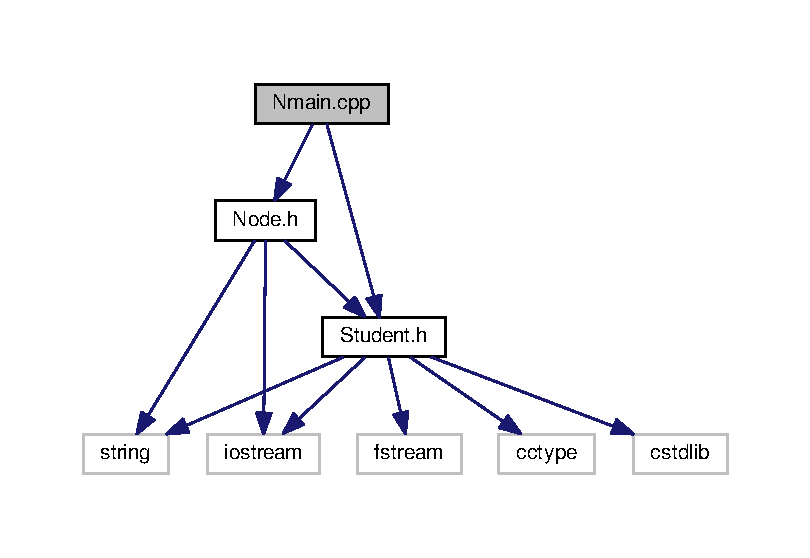
\includegraphics[width=350pt]{Nmain_8cpp__incl}
\end{center}
\end{figure}
\subsection*{Functions}
\begin{DoxyCompactItemize}
\item 
void \hyperlink{Nmain_8cpp_af8bf7d7d3b262c434aa5a55ed4bd7410}{append} (\hyperlink{classNode}{Node} $\ast$\&n, \hyperlink{classNode}{Node} $\ast$\&head)
\item 
void \hyperlink{Nmain_8cpp_a7a5e5d32951bef6994e209b048ed6acc}{display} (\hyperlink{classNode}{Node} $\ast$\&head)
\item 
bool \hyperlink{Nmain_8cpp_a50b1f8ace0b1cc448d7acc0387ca0ca6}{delete\+Node} (\hyperlink{classNode}{Node} $\ast$\&head, string target)
\item 
void \hyperlink{Nmain_8cpp_ac20747b60ed410e225f6d88ffe2edb91}{end} (\hyperlink{classNode}{Node} $\ast$\&head)
\item 
void \hyperlink{Nmain_8cpp_a70ec1382d8ba4ede7bc41284e71ba46f}{create\+Student} (string \&f, string \&l, char \&m, int \&ssn, int \&a)
\item 
int \hyperlink{Nmain_8cpp_ae66f6b31b5ad750f1fe042a706a4e3d4}{main} ()
\end{DoxyCompactItemize}


\subsection{Function Documentation}
\index{Nmain.\+cpp@{Nmain.\+cpp}!append@{append}}
\index{append@{append}!Nmain.\+cpp@{Nmain.\+cpp}}
\subsubsection[{\texorpdfstring{append(\+Node $\ast$\&n, Node $\ast$\&head)}{append(Node *&n, Node *&head)}}]{\setlength{\rightskip}{0pt plus 5cm}void append (
\begin{DoxyParamCaption}
\item[{{\bf Node} $\ast$\&}]{n, }
\item[{{\bf Node} $\ast$\&}]{head}
\end{DoxyParamCaption}
)}\hypertarget{Nmain_8cpp_af8bf7d7d3b262c434aa5a55ed4bd7410}{}\label{Nmain_8cpp_af8bf7d7d3b262c434aa5a55ed4bd7410}

\begin{DoxyCode}
70 \{
71    \hyperlink{classNode}{Node}* curr;
72    \textcolor{keywordflow}{if}(head == NULL)
73       head = n; \textcolor{comment}{//first Node added to the list                                                             
                                                                                                       }
74    \textcolor{keywordflow}{else}
75    \{
76       curr = head;
77       \textcolor{keywordflow}{while}(curr -> \hyperlink{classNode_af8f2d178f274dd254e6e1965971f0fd0}{getNext}() != NULL) \textcolor{comment}{//finds the last Node in the list                            
                                                                                                              }
78          curr = curr -> \hyperlink{classNode_af8f2d178f274dd254e6e1965971f0fd0}{getNext}();
79       curr -> \hyperlink{classNode_a0f69ba4f73cd616755f4ec0ae9fa7f96}{setNext}(n); \textcolor{comment}{//appends Node onto the end of the list                                   
                                                                                                              }
80    \}
81 \}
\end{DoxyCode}
\index{Nmain.\+cpp@{Nmain.\+cpp}!create\+Student@{create\+Student}}
\index{create\+Student@{create\+Student}!Nmain.\+cpp@{Nmain.\+cpp}}
\subsubsection[{\texorpdfstring{create\+Student(string \&f, string \&l, char \&m, int \&ssn, int \&a)}{createStudent(string &f, string &l, char &m, int &ssn, int &a)}}]{\setlength{\rightskip}{0pt plus 5cm}void create\+Student (
\begin{DoxyParamCaption}
\item[{string \&}]{f, }
\item[{string \&}]{l, }
\item[{char \&}]{m, }
\item[{int \&}]{ssn, }
\item[{int \&}]{a}
\end{DoxyParamCaption}
)}\hypertarget{Nmain_8cpp_a70ec1382d8ba4ede7bc41284e71ba46f}{}\label{Nmain_8cpp_a70ec1382d8ba4ede7bc41284e71ba46f}

\begin{DoxyCode}
56 \{
57    cout << \textcolor{stringliteral}{"Enter first name: "};
58    cin >> f;
59    cout << \textcolor{stringliteral}{"Enter last name: "};
60    cin >> l;
61    cout << \textcolor{stringliteral}{"Enter middle initial: "};
62    cin >> m;
63    cout << \textcolor{stringliteral}{"Enter social security number: "};
64    cin >> ssn;
65    cout << \textcolor{stringliteral}{"Enter age: "};
66    cin >> a;
67 \}
\end{DoxyCode}
\index{Nmain.\+cpp@{Nmain.\+cpp}!delete\+Node@{delete\+Node}}
\index{delete\+Node@{delete\+Node}!Nmain.\+cpp@{Nmain.\+cpp}}
\subsubsection[{\texorpdfstring{delete\+Node(\+Node $\ast$\&head, string target)}{deleteNode(Node *&head, string target)}}]{\setlength{\rightskip}{0pt plus 5cm}bool delete\+Node (
\begin{DoxyParamCaption}
\item[{{\bf Node} $\ast$\&}]{head, }
\item[{string}]{target}
\end{DoxyParamCaption}
)}\hypertarget{Nmain_8cpp_a50b1f8ace0b1cc448d7acc0387ca0ca6}{}\label{Nmain_8cpp_a50b1f8ace0b1cc448d7acc0387ca0ca6}

\begin{DoxyCode}
108 \{
109    \textcolor{keywordtype}{bool} del = \textcolor{keyword}{false};
110    \hyperlink{classNode}{Node}* temp = NULL;
111    \hyperlink{classNode}{Node}* curr = head;
112    \hyperlink{classNode}{Node}* \hyperlink{classNode_ac953360c5f7ffae6ad13762189d34d9c}{prev} = NULL; \textcolor{comment}{//prev starts at NULL because curr starts at head                            
                                                                                                               }
113    \textcolor{keywordflow}{while}(curr)
114    \{
115       \textcolor{keywordflow}{if}(curr->getStudent().getFirstName() != target) \textcolor{comment}{//target not found, moves to next Node               
                                                                                                       }
116       \{
117          prev = curr;
118          curr = curr -> \hyperlink{classNode_af8f2d178f274dd254e6e1965971f0fd0}{getNext}();
119       \}
120       \textcolor{keywordflow}{else}
121       \{
122          \textcolor{keywordflow}{if}(prev == NULL) \textcolor{comment}{//Node to be deleted is the first one in the list                                
                                                                                                       }
123          \{
124             head = curr -> \hyperlink{classNode_af8f2d178f274dd254e6e1965971f0fd0}{getNext}(); \textcolor{comment}{//head points to next Node                                    
                                                                                                              }
125          \}
126          \textcolor{keywordflow}{else} \textcolor{comment}{//Node is in middle of list or at the end                                                    
                                                                                                       }
127             prev -> \hyperlink{classNode_a0f69ba4f73cd616755f4ec0ae9fa7f96}{setNext}(curr -> \hyperlink{classNode_af8f2d178f274dd254e6e1965971f0fd0}{getNext}()); \textcolor{comment}{//                                           
                                                                                                                  
         }
128          curr -> deleteStudent(); \textcolor{comment}{//releases dynamically allocated memory of Student                       
                                                                                                       }
129          \textcolor{keyword}{delete} curr; \textcolor{comment}{//releases dynamically allocated memory of Node                                      
                                                                                                       }
130          curr = NULL;
131          del = \textcolor{keyword}{true}; \textcolor{comment}{//Because a Node is deleted, function sends back TRUE                                 
                                                                                                       }
132       \}
133    \}
134    \textcolor{keywordflow}{return} del;
135 \}
\end{DoxyCode}
\index{Nmain.\+cpp@{Nmain.\+cpp}!display@{display}}
\index{display@{display}!Nmain.\+cpp@{Nmain.\+cpp}}
\subsubsection[{\texorpdfstring{display(\+Node $\ast$\&head)}{display(Node *&head)}}]{\setlength{\rightskip}{0pt plus 5cm}void display (
\begin{DoxyParamCaption}
\item[{{\bf Node} $\ast$\&}]{head}
\end{DoxyParamCaption}
)}\hypertarget{Nmain_8cpp_a7a5e5d32951bef6994e209b048ed6acc}{}\label{Nmain_8cpp_a7a5e5d32951bef6994e209b048ed6acc}

\begin{DoxyCode}
84 \{
85    \hyperlink{classNode}{Node}* curr = head;
86    cout << endl;
87    \textcolor{keywordflow}{while}(curr != NULL) \textcolor{comment}{//goes through all Nodes                                                            
                                                                                                       }
88    \{
89       cout << curr -> getStudent() << endl; \textcolor{comment}{//displays Student information}
90      curr = curr -> \hyperlink{classNode_af8f2d178f274dd254e6e1965971f0fd0}{getNext}(); \textcolor{comment}{//goes to the next Node in the list                                  
                                                                                                             }
91    \}
92 \}
\end{DoxyCode}
\index{Nmain.\+cpp@{Nmain.\+cpp}!end@{end}}
\index{end@{end}!Nmain.\+cpp@{Nmain.\+cpp}}
\subsubsection[{\texorpdfstring{end(\+Node $\ast$\&head)}{end(Node *&head)}}]{\setlength{\rightskip}{0pt plus 5cm}void end (
\begin{DoxyParamCaption}
\item[{{\bf Node} $\ast$\&}]{head}
\end{DoxyParamCaption}
)}\hypertarget{Nmain_8cpp_ac20747b60ed410e225f6d88ffe2edb91}{}\label{Nmain_8cpp_ac20747b60ed410e225f6d88ffe2edb91}

\begin{DoxyCode}
95 \{
96    \hyperlink{classNode}{Node}* curr = head;
97    \hyperlink{classNode}{Node}* del;
98    \textcolor{keywordflow}{while}(curr != NULL)
99    \{
100       del = curr;
101       curr -> deleteStudent(); \textcolor{comment}{//releases the Student memory of the Node                                   
                                                                                                       }
102       curr = curr -> \hyperlink{classNode_af8f2d178f274dd254e6e1965971f0fd0}{getNext}();
103       \textcolor{keyword}{delete} del; \textcolor{comment}{//releases the Node memory                                                               
                                                                                                       }
104    \}
105 \}
\end{DoxyCode}
\index{Nmain.\+cpp@{Nmain.\+cpp}!main@{main}}
\index{main@{main}!Nmain.\+cpp@{Nmain.\+cpp}}
\subsubsection[{\texorpdfstring{main()}{main()}}]{\setlength{\rightskip}{0pt plus 5cm}int main (
\begin{DoxyParamCaption}
{}
\end{DoxyParamCaption}
)}\hypertarget{Nmain_8cpp_ae66f6b31b5ad750f1fe042a706a4e3d4}{}\label{Nmain_8cpp_ae66f6b31b5ad750f1fe042a706a4e3d4}

\begin{DoxyCode}
21 \{
22    \hyperlink{classNode}{Node}* head = NULL;
23    \hyperlink{classNode}{Node}* nPtr;
24    \textcolor{keywordtype}{string} f, l;
25    \textcolor{keywordtype}{int} n, ssn, a;
26    \textcolor{keywordtype}{char} ans, m;
27    \textcolor{keywordtype}{bool} del;
28 
29    \textcolor{keywordflow}{do}
30    \{
31       \hyperlink{Nmain_8cpp_a70ec1382d8ba4ede7bc41284e71ba46f}{createStudent}(f, l, m, ssn, a);
32       nPtr = \textcolor{keyword}{new} \hyperlink{classNode_a0ac1d44cfe588be564acf25485029bd8}{Node}(f, l, m, ssn, a); \textcolor{comment}{//creates new Node (which nPtr points to) with the Student
       object just created                                                                                      }
33       \hyperlink{Nmain_8cpp_af8bf7d7d3b262c434aa5a55ed4bd7410}{append}(nPtr, head); \textcolor{comment}{//appends the newly created Node to the list                               
                                                                                                             }
34       cout << \textcolor{stringliteral}{"\(\backslash\)nAdd a new student to the list? y/n: "};
35       cin >> ans;
36       cout << endl;
37    \}\textcolor{keywordflow}{while}(ans == \textcolor{charliteral}{'y'} || ans == \textcolor{charliteral}{'Y'}); \textcolor{comment}{//Nodes will be created until user does not enter y or Y              
                                                                                                       }
38 
39    cout << \textcolor{stringliteral}{"Student list:"} << endl;
40    \hyperlink{Nmain_8cpp_a7a5e5d32951bef6994e209b048ed6acc}{display}(head); \textcolor{comment}{//displays list                                                                   
                                                                                                              }
41 
42    \textcolor{keywordflow}{do}
43    \{
44       del = \hyperlink{Nmain_8cpp_a50b1f8ace0b1cc448d7acc0387ca0ca6}{deleteNode}(head, \textcolor{stringliteral}{"Christine"}); \textcolor{comment}{//deletes all Nodes with the name Christine           
                                                                                                                 }
45    \}\textcolor{keywordflow}{while}(del); \textcolor{comment}{//continue to delete Nodes until there are no more Christines in the list                  
                                                                                                       }
46 
47    cout << \textcolor{stringliteral}{"After Christine has been deleted from list:"} << endl;
48    \hyperlink{Nmain_8cpp_a7a5e5d32951bef6994e209b048ed6acc}{display}(head);
49    \hyperlink{Nmain_8cpp_ac20747b60ed410e225f6d88ffe2edb91}{end}(head);
50    \textcolor{keywordflow}{return} 0;
51 \}
\end{DoxyCode}


Here is the call graph for this function\+:
\nopagebreak
\begin{figure}[H]
\begin{center}
\leavevmode
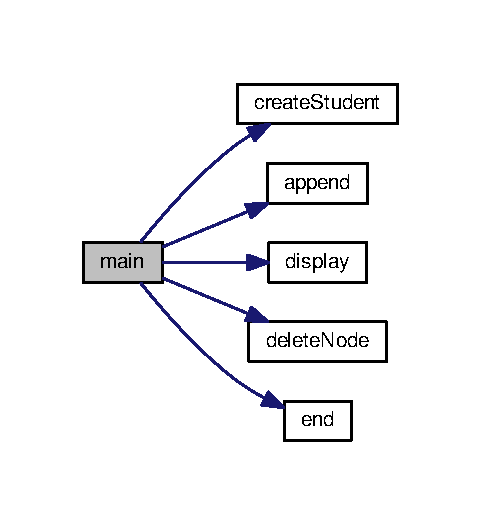
\includegraphics[width=231pt]{Nmain_8cpp_ae66f6b31b5ad750f1fe042a706a4e3d4_cgraph}
\end{center}
\end{figure}



\hypertarget{Node_8cpp}{}\section{Node.\+cpp File Reference}
\label{Node_8cpp}\index{Node.\+cpp@{Node.\+cpp}}
{\ttfamily \#include \char`\"{}Node.\+h\char`\"{}}\\*
{\ttfamily \#include \char`\"{}Student.\+h\char`\"{}}\\*
Include dependency graph for Node.\+cpp\+:
\nopagebreak
\begin{figure}[H]
\begin{center}
\leavevmode
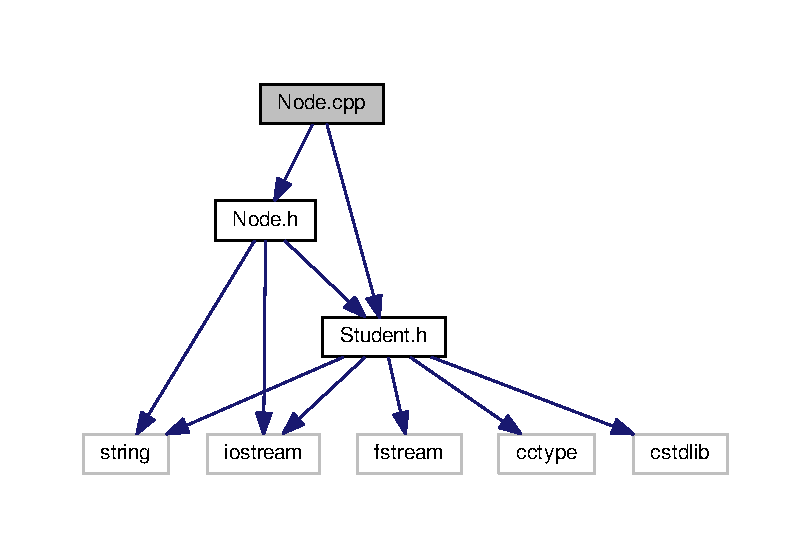
\includegraphics[width=350pt]{Node_8cpp__incl}
\end{center}
\end{figure}

\hypertarget{Node_8h}{}\section{Node.\+h File Reference}
\label{Node_8h}\index{Node.\+h@{Node.\+h}}
{\ttfamily \#include $<$iostream$>$}\\*
{\ttfamily \#include $<$string$>$}\\*
{\ttfamily \#include \char`\"{}Student.\+h\char`\"{}}\\*
Include dependency graph for Node.\+h\+:
\nopagebreak
\begin{figure}[H]
\begin{center}
\leavevmode
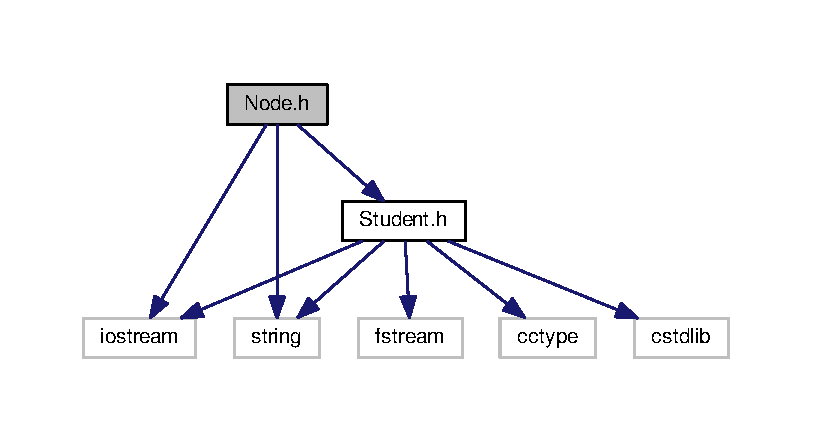
\includegraphics[width=350pt]{Node_8h__incl}
\end{center}
\end{figure}
This graph shows which files directly or indirectly include this file\+:
\nopagebreak
\begin{figure}[H]
\begin{center}
\leavevmode
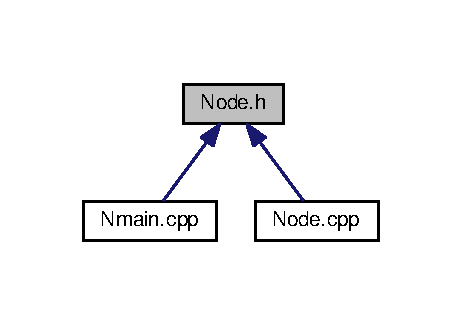
\includegraphics[width=350pt]{Node_8h__dep__incl}
\end{center}
\end{figure}
\subsection*{Classes}
\begin{DoxyCompactItemize}
\item 
class \hyperlink{classNode}{Node$<$ T $>$}
\end{DoxyCompactItemize}

\hypertarget{Student_8cpp}{}\section{Student.\+cpp File Reference}
\label{Student_8cpp}\index{Student.\+cpp@{Student.\+cpp}}
{\ttfamily \#include \char`\"{}Student.\+h\char`\"{}}\\*
Include dependency graph for Student.\+cpp\+:
\nopagebreak
\begin{figure}[H]
\begin{center}
\leavevmode
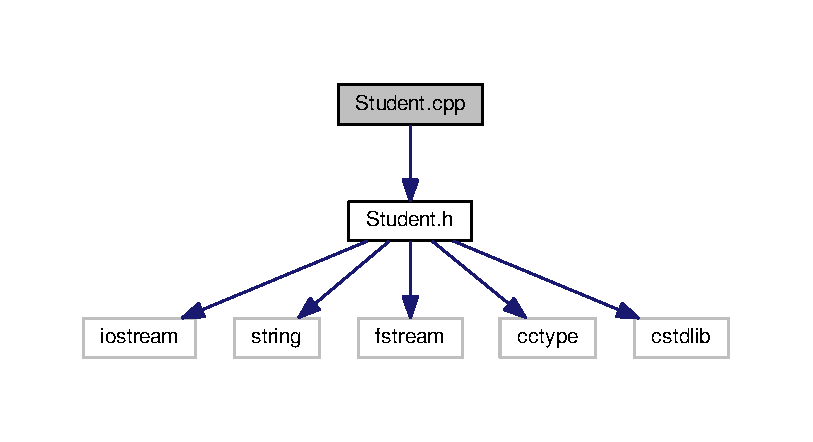
\includegraphics[width=350pt]{Student_8cpp__incl}
\end{center}
\end{figure}
\subsection*{Functions}
\begin{DoxyCompactItemize}
\item 
ostream \& \hyperlink{Student_8cpp_a8ed16acc8384ea29641694cb182ac764}{operator$<$$<$} (ostream \&outs, const \hyperlink{classStudent}{Student} \&s)
\item 
istream \& \hyperlink{Student_8cpp_a2d76cee765e6e0d66e66a27d10fa0a68}{operator$>$$>$} (istream \&ins, \hyperlink{classStudent}{Student} \&s)
\end{DoxyCompactItemize}


\subsection{Function Documentation}
\index{Student.\+cpp@{Student.\+cpp}!operator$<$$<$@{operator$<$$<$}}
\index{operator$<$$<$@{operator$<$$<$}!Student.\+cpp@{Student.\+cpp}}
\subsubsection[{\texorpdfstring{operator$<$$<$(ostream \&outs, const Student \&s)}{operator<<(ostream &outs, const Student &s)}}]{\setlength{\rightskip}{0pt plus 5cm}ostream\& operator$<$$<$ (
\begin{DoxyParamCaption}
\item[{ostream \&}]{outs, }
\item[{const {\bf Student} \&}]{s}
\end{DoxyParamCaption}
)}\hypertarget{Student_8cpp_a8ed16acc8384ea29641694cb182ac764}{}\label{Student_8cpp_a8ed16acc8384ea29641694cb182ac764}

\begin{DoxyCode}
65 \{
66    cout << \textcolor{stringliteral}{"Student:\(\backslash\)t\(\backslash\)t  "} << s.\hyperlink{classStudent_a6c934004d6a468a354916bcf0f998190}{lname} << \textcolor{stringliteral}{", "} << s.\hyperlink{classStudent_a333c7d227c87fdfa821d0232e21f9006}{fname} << \textcolor{stringliteral}{" "} << s.
      \hyperlink{classStudent_afd8d4557f2ac6bb7681c32e691248328}{mi} << endl;
67    cout << \textcolor{stringliteral}{"Social Security number:\(\backslash\)t  "} << s.\hyperlink{classStudent_aa7181a8aac86888176481f901bee2cbd}{ssn} << endl;
68    cout << \textcolor{stringliteral}{"Age:\(\backslash\)t\(\backslash\)t\(\backslash\)t  "} << s.\hyperlink{classStudent_a552a431a43ffc545d180424597d51f97}{age} << endl;
69    cout << \textcolor{stringliteral}{"------------------------------------------------------"} << endl;
70 
71    \textcolor{keywordflow}{return} outs;
72 \}
\end{DoxyCode}
\index{Student.\+cpp@{Student.\+cpp}!operator$>$$>$@{operator$>$$>$}}
\index{operator$>$$>$@{operator$>$$>$}!Student.\+cpp@{Student.\+cpp}}
\subsubsection[{\texorpdfstring{operator$>$$>$(istream \&ins, Student \&s)}{operator>>(istream &ins, Student &s)}}]{\setlength{\rightskip}{0pt plus 5cm}istream\& operator$>$$>$ (
\begin{DoxyParamCaption}
\item[{istream \&}]{ins, }
\item[{{\bf Student} \&}]{s}
\end{DoxyParamCaption}
)}\hypertarget{Student_8cpp_a2d76cee765e6e0d66e66a27d10fa0a68}{}\label{Student_8cpp_a2d76cee765e6e0d66e66a27d10fa0a68}

\begin{DoxyCode}
75 \{
76    ins >> s.\hyperlink{classStudent_a333c7d227c87fdfa821d0232e21f9006}{fname} >> s.\hyperlink{classStudent_a6c934004d6a468a354916bcf0f998190}{lname} >> s.\hyperlink{classStudent_afd8d4557f2ac6bb7681c32e691248328}{mi} >> s.\hyperlink{classStudent_aa7181a8aac86888176481f901bee2cbd}{ssn} >> s.\hyperlink{classStudent_a552a431a43ffc545d180424597d51f97}{age};
77 \}
\end{DoxyCode}

\hypertarget{Student_8h}{}\section{Student.\+h File Reference}
\label{Student_8h}\index{Student.\+h@{Student.\+h}}
{\ttfamily \#include $<$iostream$>$}\\*
{\ttfamily \#include $<$string$>$}\\*
{\ttfamily \#include $<$fstream$>$}\\*
{\ttfamily \#include $<$cctype$>$}\\*
{\ttfamily \#include $<$cstdlib$>$}\\*
Include dependency graph for Student.\+h\+:
\nopagebreak
\begin{figure}[H]
\begin{center}
\leavevmode
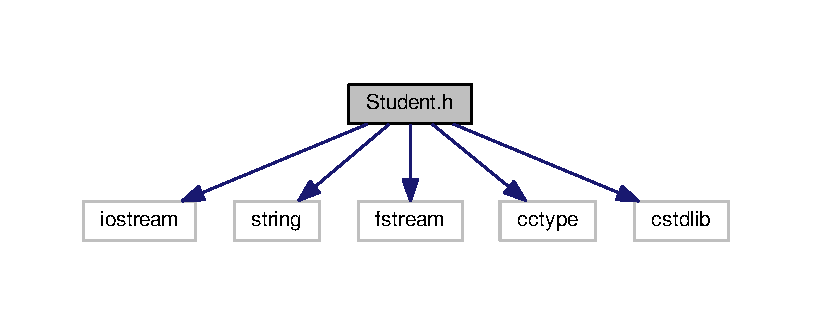
\includegraphics[width=350pt]{Student_8h__incl}
\end{center}
\end{figure}
This graph shows which files directly or indirectly include this file\+:
\nopagebreak
\begin{figure}[H]
\begin{center}
\leavevmode
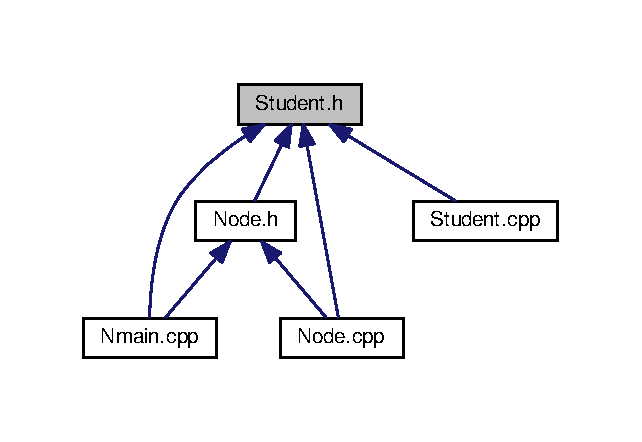
\includegraphics[width=308pt]{Student_8h__dep__incl}
\end{center}
\end{figure}
\subsection*{Classes}
\begin{DoxyCompactItemize}
\item 
class \hyperlink{classStudent}{Student}
\end{DoxyCompactItemize}

%--- End generated contents ---

% Index
\backmatter
\newpage
\phantomsection
\clearemptydoublepage
\addcontentsline{toc}{chapter}{Index}
\printindex

\end{document}
